\chapter{Des atomes de Rydberg circulaires sur puce}
\label{chapter:50c}
%Excitation d'atomes de Rydberg circulaires et piégeage laser
\vfill
\minitoc
\newpage

\noindent La première étape vers la réalisation de notre proposition de simulateur quantique est l'excitation d'atomes de Rydberg circulaires près de la puce à atomes.
Ceux-ci sont obtenus par passage adiabatique rapide, grâce à un champ radio-fréquence polarisé,  à partir de niveaux de Rydberg de bas moment cinétique excités par laser.
Le principe de cette excitation est résumé en figure \eqref{fig:levels_circ}

\begin{figure}[h]
\centering
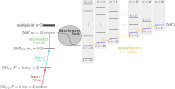
\includegraphics[width=\linewidth]{figures/circulars/level_scheme_5S50C}
\caption[Schéma de niveaux pour l'excitation d'atomes de Rydberg circulaires]
{Schéma de niveaux pour l'excitation d'atomes de Rydberg circulaires.
Un impulsion laser à deux photons excite le niveau $\mathrm{50D}$ depuis le niveau fondamental $\mathrm{5S}$.
%Un champ électrique de $\SI{2.35}{\V/\cm}$ est imposé, qui permet de passer dans la base parabolique $\ket{n,m,k}$.
Une impulsion microonde transfère les atomes dans le niveau $\mathrm{50F},m=2$.
Le branchement Stark consiste en l'allumage adiabatique d'un champ électrique qui transfère le niveau $\mathrm{50F},m=2$ de la base sphérique vers le niveau $\ket{n=50,m=2,k=-45}$ de la base parabolique.
Enfin, un passage adiabatique rapide amène les atomes dans le niveau circulaire $\mathrm{50C}$.
}\label{fig:levels_circ}
\end{figure}

Dans ce chapitre, nous présenterons le principe du passage adiabatique de circularisation et les modifications que nous avons apportées au dispositif expérimental afin de pouvoir le mettre en \oe uvre.
Nous décrirons et caractériserons ensuite chaque étape de l'excitation depuis le niveau fondamental jusqu'au niveau de Rydberg circulaire.
Nous montrerons les premiers résultats expérimentaux mettant en évidence, par spectroscopie microonde, l'excitation d'atomes de Rydberg circulaires près d'une puce.

\section{Principe du passage adiabatique}
 \subsection{Le passage adiabatique idéal pour l'atome d'hydrogène}
\noindent Les niveaux de Rydberg de grand moment cinétique ne sont pas accessibles par excitation laser.
En effet, une excitation laser à deux photons depuis le niveau $\mathrm{5S}$ ne peut au maximum amener les atomes que dans un état de moment cinétique $l=2$\footnote{
Des dispositifs d'excitation à trois lasers peuvent être mis en place mais le problème reste entier.
}.
Il faut donc trouver un moyen d'augmenter le moment cinétique d'un atome en gardant constant son nombre quantique principal $n$.
L'effet Stark permet de lever la dégénérescence des différents niveaux $\ket{n,m,k}$ d'une même multiplicité.
L'échelle de niveaux correspondante est représentée, pour l'atome d'hydrogène, en figure \eqref{fig:sigmap_hydrogen}.
%
\begin{figure}[t]
\centering
\includegraphics[width=.6\linewidth]{figures/circulars/sigmap_hydrogen}
\caption[Échelle des niveaux Stark de l'atome d'hydrogène]{
Échelle des niveaux Stark de l'atome d'hydrogène.
Un champ radio-fréquence polarisé $\sigma^+$ permet de coupler les niveaux de la diagonale du bas, représentés en bleu.
}
\label{fig:sigmap_hydrogen}
\end{figure} 
%
Au premier ordre, les niveaux $\ket{n,m,k}$ et $\ket{n,m+1,k+1}$ sont séparés d'une énergie
\begin{equation}
h\nu_{RF^+}(F) = \frac{3}{2}n|\vec{F}|\times ea_0 , %2E_I,
\end{equation}
où $\vec{F}$ est le champ électrique. % et $E_I$ l'énergie d'ionisation.
Pour $n=50$ et un champ électrique de $\SI{2}{\V/cm}$, cette énergie est de l'ordre de $h\times\SI{200}{\MHz}$.
Les niveaux $\ket{n,m,k}$ et $\ket{n,m+1,k+1}$ peuvent ainsi être couplés par un champ radio-fréquence $\sigma^+$ à la fréquence $\nu_{RF^+}(F)$.
Une série de $n-1$ photons $\sigma^+$ à la fréquence $\nu_{RF^+}(F)$ permettrait donc de transférer un atome du niveau $\ket{n,m=0,k=-(n-1)}$ jusqu'au niveau circulaire $\ket{\mathrm{nC}}=\ket{n,m=n-1,k=0}$.

Une approche plus robuste consiste à effectuer ce transfert par passage adiabatique.
Cette technique s'explique intuitivement dans le formalisme de l'atome habillé.
Habillons donc notre atome d'hydrogène, avec un champ radio-fréquence $\sigma^+$ à la fréquence $\nu_{RF^+}(F_0)$, où $F_0$ est une valeur arbitraire du champ électrique.
Nous obtenons le diagramme de niveaux présenté en figure (\ref{fig:passage_adiab_hydrogen} a), représentant l'énergie des niveaux habillés $\ket{n,m,p}$ où $p$ est le nombre de photons radio-fréquence absorbés et où le nombre quantique $k$ est omis car toujours minimal.
%
\begin{figure}[h]
\centering
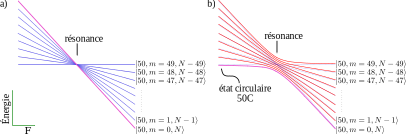
\includegraphics[width=\linewidth]{figures/circulars/passage_adiab_hydrogen}
\caption[Principe du passage adiabatique de circularisation]{
Principe du passage adiabatique de circularisation.
\textbf{a)} Diagramme d'énergie de l'atome habillé, sans couplage avec le champ RF.
En augmentant le champ électrique $F$, le niveau habillé $\ket{n,0,N}$ suit les flèches roses.
\textbf{b)} Diagramme d'énergie de l'atome habillé, couplé au champ RF.
En diminuant le champ électrique, le niveau habillé $\ket{n,0,N}$ suit les flèches roses vers le niveau habillé $\ket{n,n-1,N-(n-1)}$. \`A l'extinction du champ RF, celui-ci est branché sur le niveau circulaire $\ket{\mathrm{nC}}$.
}
\label{fig:passage_adiab_hydrogen}
\end{figure} 
%
En augmentant le champ électrique $F$ jusqu'à une valeur $F_{max}>F_0$, l'état $\ket{n,m=0,N}$ traverse la résonance $F=F_0$.
En allumant le champ radio-fréquence% avec une fréquence de Rabi $\Omega_{RF}$
, le croisement à résonance des niveaux habillés devient un anti-croisement, représenté en figure (\ref{fig:passage_adiab_hydrogen} b).
En diminuant adiabatiquement la valeur du champ électrique, le niveau $\ket{n,m=0,N}$ est transféré vers le niveau $\ket{n,m=n-1,N-(n-1)}$ lors du passage par la résonance.
Enfin, l'extinction du champ radio-fréquence branche le niveau $\ket{n,m=n-1,N-(n-1)}$ sur le niveau circulaire $\ket{\mathrm{nC}}$.


 \subsection{Le passage adiabatique avec défaut quantique}\label{subsec:adiab_Qdefect}
\noindent Malheureusement, le défaut quantique du rubidium déplace les niveaux de faible $l$ et les niveaux situés en bas de l'échelle Stark ne sont plus couplés au reste de la multiplicité par le champ radio-fréquence à $\nu_{RF^+}$.
Le niveau le plus bas qui puisse être couplé à la multiplicité se trouve être le niveau $\ket{n,m=2,k=2-(n-1)+2}$, que nous noterons $\ket{n,2,k_0}$.
%Pour un champ électrique $F_0=\SI{2.4}{\V/\cm}$, la fréquence $\nu_{RF^+}$ vaut $\SI{230}{\MHz}$, et $\ket{n,2,k_0}$ est séparé de $\ket{n,3,k_0+1}$ par une énergie $h\times\SI{230}{\MHz}$.
Le passage adiabatique de circularisation pour le rubidium, représenté en figure \eqref{fig:levels_circ}, commencera donc dans ce niveau.

Il nous faut maintenant savoir comment exciter ce niveau de départ.
\`A bas $l$, le défaut quantique est important et un très grand champ électrique serait nécessaire pour que les bons nombres quantiques deviennent $\ket{n,m,k}$ au lieu de $\ket{n,l,m}$.
Nous pouvons alors identifier quel niveau $\ket{n,l_0,m_0}$ a la plus grande projection sur $\ket{n,2,k_0}$, puis allumer progressivement le champ électrique afin de brancher adiabatiquement $\ket{n,l_0,m_0}$ sur $\ket{n,2,k_0}$.
Or le niveau $\ket{n,l_0,m_0}$ se trouve être le niveau $\ket{n,l=3,m=2}=\ket{nF,m=2}$.

Ainsi, afin d'exciter le niveau circulaire $\mathrm{50C}$, nous devrons exciter le niveau $\ket{50F,m=2}$ puis lui faire subir un passage adiabatique radio-fréquence.
Puisque nous disposons de deux lasers pour l'excitation des niveaux de Rydberg, nous ne pouvons adresser par laser la transition $\mathrm{5S}\rightarrow\mathrm{50F}$.
Nous devrons donc exciter par laser le niveau $\mathrm{50D}$, puis transférer celui-ci vers le niveau $\mathrm{50F}$ par une impulsion microonde.
Cette suite de transitions menant au niveau circulaire est résumée en figure \ref{fig:levels_circ}.

\section{Modifications du dispositif expérimental}

\noindent La réalisation du passage adiabatique de circularisation nécessite de pouvoir imposer un champ électrique radio-fréquence tournant au niveau des atomes.
De plus, les niveaux de Rydberg circulaires ont un seuil d'ionisation des champs bien plus élevés que les niveaux de Rydberg de bas $l$\cite{TXT_GALLAGHER}.
En raison de ces deux particularités, nous avons dû apporter des modifications au dispositif expérimental.

 \subsection{Contrôle du champ parallèle à la puce}% et électrodes RF de circularisation}
\noindent Le dispositif de contrôle des champs électriques dont nous disposions auparavant, présenté au chapitre \ref{chapter:setup_coldatoms_Rydberg}, ne permettait de varier le champ électrique que perpendiculairement à la puce, soit dans la direction $y$.
Un champ électrique statique $F$ est imposé par ce dispositif, qui définit l'axe de quantification du moment cinétique des atomes selon $Oy$.
Afin de réaliser le passage adiabatique de circularisation, nous avons besoin de contrôler le champ dans le plan $xOz$, c'est-à-dire parallèlement à la puce. 

Notre dispositif de contrôle du champ parallèle à la puce consiste en quatre électrodes cylindriques (\og électrodes RF \fg{}) , disposées en carré autour de la zone de piégeage des atomes.
En appliquant à ces électrodes des tensions oscillantes avec des phases bien optimisées, nous pourrons générer un champ électrique radio-fréquence arbitrairement polarisé au niveau des atomes.
En appliquant des tensions constantes arbitraires sur ces électrodes, nous pourrons aussi compenser les champs résiduels dans les directions $x$ et $z$.

La figure \ref{fig:RF_ELECTRODES} montre la disposition de ces électrodes au c\oe ur du dispositif expérimental.
%
\begin{figure}[!h]
\centering
\includegraphics[width=.4\linewidth]{figures/setup/rydberg/electrodes_RF_3D_labeled.jpg}
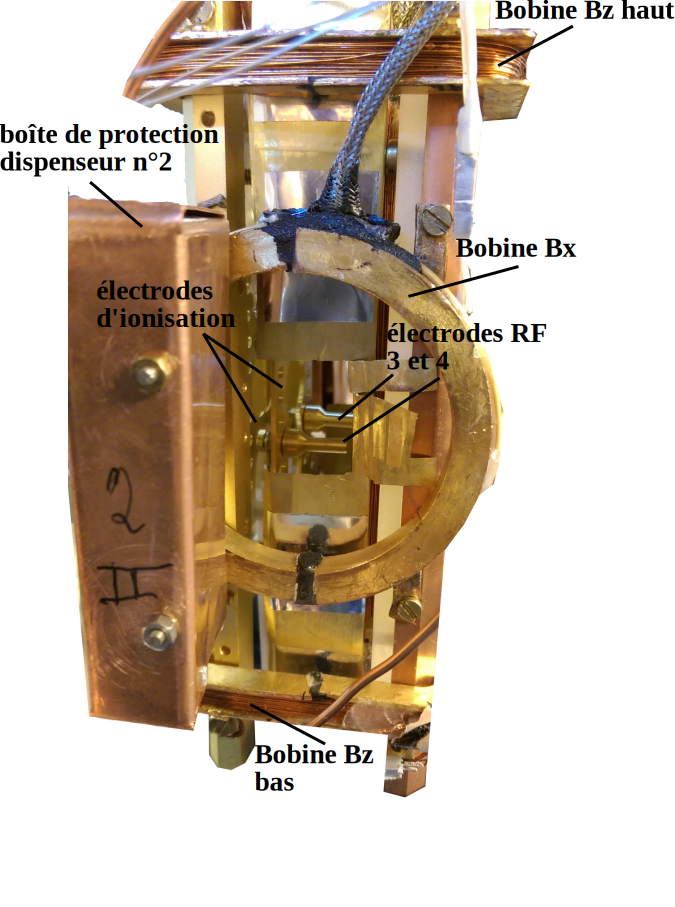
\includegraphics[width=.4\linewidth]{figures/setup/rydberg/electrodes_RF_photo}
\caption[Électrodes de circularisation et de contrôle du champ parallèle]{
Électrodes \og RF \fg{} de circularisation et de contrôle du champ parallèle à la puce.
\`A gauche, schéma représentant les électrodes RF, fixées sur l'électrode d'ionisation $I_1$, et numérotées de $1$ à $4$.
\`A droite, photographie du c\oe ur de l'expérience.
On y voit la \og boîte \fg{} de protection de l'un des dispenseurs de rubidium, les bobines de biais $B_z$ et l'une des bobines de biais $B_x$, les deux électrodes d'ionisation, et les deux électrodes RF du bas (3 et 4).
}
\label{fig:RF_ELECTRODES}
\end{figure}
%

\subsubsection*{Description technique du dispositif}
\noindent Chaque électrode RF est un cylindre de $\SI{6}{\mm}$ de diamètre et de $\SI{12}{\mm}$ de long, en cuivre doré.
Les quatre cylindres sont disposés perpendiculairement à la puce en un carré de $\SI{30}{\mm}$ de côté.
Afin de fixer les cylindres au sein du dispositif, nous avons percé des trous dans l'électrode d'ionisation $I_1$.
Chaque électrode est fixée par une tige filetée traversant l'un de ces trous et maintenue par un écrou.
Or les électrodes RF doivent être isolées de l'électrode $I_1$.
Les écrous de fixation sont ainsi isolés de $I_1$ par des rondelles en nylon.
Les tiges filetées sont quant à elles isolées par des espaceurs en céramique MACOR, logés dans la base élargie et évidée de chaque cylindre et traversant l'électrode $I_1$.
Le recouvrement de ces pièces diélectriques par les électrodes elles-mêmes est crucial, afin de limiter au maximum l'exposition des atomes à des surfaces non-conductrices susceptibles d'emmagasiner des charges électriques et de créer ainsi des champs parasites.
La longueur des cylindres en cuivre et l'épaisseur des espaceurs en céramique sont calculés pour que le bout de chaque cylindre arrive à une distance d'environ $\SI{2}{\mm}$ de la surface de la puce.

La tension appliquée à chacune des électrodes RF est amenée \textit{via} des câbles coaxiaux,  permettant de propager des signaux radio-fréquence aussi bien que des tensions constantes.
Ces câbles coaxiaux semi-rigides fins traversent le cryostat, sont thermalisés à $\SI{4.2}{\K}$ au fond de la jupe hélium.
\`A l'approche du c\oe ur de l'expérience, ils sont terminées par des connecteurs SMA, auxquels viennent se brancher des câbles plus courts et plus épais.
Cette deuxième section de câblage a deux intérêts.
Premièrement, la connexion des câbles aux cosses qui sont en contact avec les électrodes est facilitée par l'épaisseur et la solidité de ces deuxièmes câbles.
Ces cosses sont intercalées entre l'écrou de fixation de chaque électrode et un second écrou de blocage, qui garantit le contact électrique avec la tige filetée et ainsi avec l'électrode.
Deuxièmement, cela nous permet, au prix d'une simple déconnexion de connecteurs SMA, de démonter ou ajuster indépendamment les câbles coaxiaux semi-rigides et le porte-puce assorti de ses électrodes.
%La construction de ce dispositif a été l'occasion de repenser le système de fixation des électrodes d'ionisation.
%Celles-ci sont désormais fixées directement au porte-puce, par l'intermédiaire d'espaceurs métalliques isolés. Cela a permis de stabiliser le montage et la distance séparant les différents éléments.

Les tensions constantes appliquées aux électrodes sont fournies par une source analogique contrôlée par ordinateur, dont les sorties sont filtrées par un circuit RC de temps caractéristique $\tau=\SI{1}{\us}$.
Cela permet de réduire le bruit électrique de cette source à une amplitude inférieure à $\SI{5}{\milli\V}_{\mathrm{pp}}$.

\subsubsection*{Simulation du champ créé par les électrodes RF}
\noindent Il était important, afin de bien concevoir la géométrie de ces électrodes RF, de savoir quel serait l'effet des tensions appliquées dessus en termes de champ électrique au niveau des atomes.
L'estimation du champ créé ne peut pas se faire simplement par les approximations de conducteurs infinis pour lesquels il suffirait de diviser la différence de potentiel entre eux par la distance les séparant.
En effet, la géométrie des électrodes est assez éloignée de ce genre de modèle et limite ainsi la validité qu'aurait une telle approximation.
De plus, la région où nous souhaitons créer du champ électrique est très proche de la puce, entre $\SI{0.5}{}$ et $\SI{2}{\mm}$ de celle-ci.
C'est-à-dire que d'une part cette région est située en dehors du volume délimité par les quatre électrodes, et d'autre part que la présence proche d'une surface conductrice considérée comme infinie (la puce) perturbera grandement les lignes de champ dans cette région.

Afin d'estimer le champ créé par les électrodes, nous avons utilisé le logiciel SIMION, destiné au calcul de potentiels et champs électriques et de trajectoires de particules chargées dans des structures arbitraires.
Les éléments que nous y avons programmés sont les suivants : la surface de la puce, les électrodes RF et les électrodes d'ionisation.
Cette structure simplifiée est représentée en figure \eqref{fig:RF_elec_SIMION}.
%
\begin{figure}[!h]
\centering
\includegraphics[width=\linewidth]{figures/setup/rydberg/RF_electrodes_Simion}
\caption[Électrodes de circularisation et de contrôle du champ parallèle]{
Électrodes \og RF \fg{} et leur environnement tels que programmés dans nos simulations SIMION.
Les quatre électrodes RF sont représentées, dans l'ordre de leur numérotation, en bleu foncé (1), rose (2), violet (3) et bleu turquoise (4).
La puce est représentée par une surface jaune, et les électrodes d'ionisation en vert clair ($I_1$) et vert foncé ($I_2$).
Les axes indiqués par les lettres $X$, $Y$ et $Z$ sont les axes que nous utilisons habituellement, bien que l'origine $O$ du repère ne soit pas la même.
Par souci de clarté visuelle, la figure de gauche représente les électrodes RF et d'ionisation sans la puce, et la figure de droite représente les électrodes RF et la puce, sans les électrodes d'ionisation.
}
\label{fig:RF_elec_SIMION}
\end{figure}
%

Nous présentons ci-dessous un exemple de simulation où l'on applique les potentiels suivants :
$\SI{+10}{\V}$ sur les deux électrodes RF du haut (1 et 2), $\SI{-10}{\V}$ sur les deux électrodes RF du bas (3 et 4), et $\SI{0}{\V}$ à la puce et aux électrodes d'ionisation.
%\begin{tabular}{cc}
%$10$ & $10$\\
%$-10$ & $-10$
%\end{tabular}
On espère alors appliquer un champ électrique vertical dirigé vers le bas au niveau des atomes.

La figure \eqref{fig:simion_fullregion} présente le résultat de la simulation.
%
\begin{figure}[!h]
\centering
\includegraphics[width=\linewidth]{figures/setup/rydberg/simion_4quadrants}
\caption[Champ électrique créé par les électrodes RF]{
Champ électrique créé par les électrodes RF, dans le plan $(yOz),x=0$. Les échelles de longueur en $y$ et en $z$ sont différentes.
\`A gauche la composante $F_z$, à droite la composante $F_x$.
En haut, une grande région est représentée, sur laquelle sont marquées la puce et les électrodes d'ionisation(les traits épais sont les endroits où ces électrodes sont dans le plan $(x=0)$ et les traits fins sont la projection des électrodes entières sur ce plan). Les projections des électrodes RF sur le plan $(x=0)$ sont représentées en filigrane gris (rectangles), de même que la zone de piégeage des atomes (petit ovale proche de la puce).
En bas, une région beaucoup plus petite est représentée, englobant la région typique de piégeage des atomes, représentée en filigrane gris.
\`A des fins de lisibilité, les échelles de couleur sont différentes sur chacun des graphes.
}
\label{fig:simion_fullregion}
\end{figure}
%
Les deux graphes à grande échelle (en haut), permettent de confirmer que le champ créé est largement selon $z$.
En effet, la composante $F_z$ varie de $\SIrange{+3}{-5}{\V/\cm}$ lorsque la composante $F_x$ varie de $\SIrange{-0.08}{+0.08}{\V/\cm}$.
L'on retrouve le comportement idéal des conducteurs infinis dans la zone au centre des électrodes RF, autour du point $(y= \SI{8}{\mm}, z=\SI{0}{})$ : le champ y est homogène avec des valeurs de $F_z=\SI{-5}{\V/\cm}$ et $F_x=0$.
Malheureusement, nous piégeons habituellement les atomes bien plus près de la puce, à des distance comprises entre $y=\SI{0.3}{\mm}$ et $y=\SI{1.5}{\mm}$.
Il est donc important de vérifier que, dans nos régions habituelles de piégeage, notre dispositif sera suffisamment performant.
Les deux graphes à petite échelle (en bas), nous confirment cela :
nous serons capables de créer un champ de l'ordre de $F_z=\SIrange{-0.5}{-1.5}{\V/\cm}$, avec une composante $F_x$ quasi-nulle, de l'ordre du $\SI{}{\milli\V/\cm}$.

La symétrie de la structure en $x$ et en $z$ est un argument suffisant pour affirmer que nous pourrons tout aussi bien créer un champ opposé à celui-ci, c'est-à-dire avec une composant $F_z$ positive, ou encore un champ très largement orienté selon $x$.
Nous avons néanmoins occulté dans notre description un effet indésirable :
les électrodes RF créent également un champ selon $y$ dans la région qui les sépare de la puce.
Les atomes étant piégés dans cette région, délimitée par $\num{0} < y \leq \SI{2}{\mm}$, ils subiront un champ $F_y$ dû à ces électrodes.
Dans les mêmes conditions de tensions appliquées, le champ $F_y$ varie selon $z$, dans un intervalle compris entre $\SI{-0.4}{\V/\cm}$ en $z=\SI{+0.4}{\mm}$ et $\SI{+0.4}{\V/\cm}$ en $z=\SI{-0.5}{\mm}$.
Fort heureusement le champ $F_y$ reste suffisamment homogène à l'échelle de taille des nuages atomiques de diamètre $\Delta z < \SI{300}{\um}$, une taille qui est atteinte dès le stade de mélasse optique.
De plus, nous pouvons compenser sa valeur moyenne grâce aux électrodes d'ionisation, comme nous l'avons expliqué en \ref{subsec:compensation}.

Enfin, la simulation confirme que nous pourrons appliquer un champ radio-fréquence tournant dans le plan $(xOz)$ perpendiculaire à la puce, en vue de la circularisation des atomes de Rydberg sous un champ statique selon $y$.
En effet, une différence de potentiel entre les électrodes du haut (1 et 2) et celles du bas (3 et 4) crée un champ $F_z$ quasi-pur et une différence de potentiel entre les électrodes de gauche (1 et 3) et celles de droite (2 et 4) crée un champ $F_x$ quasi-pur.
Le détail des champs tournants pour la circularisation sera discuté au chapitre \ref{chapter:50c}.

%EN VRAI, MERDE ! Gros gradients de champ selon E_y quand on est près de la puce !!

\subsection{Contrôle du champ perpendiculaire à la puce}
%Second circuit de contrôle de la tension d'ionisation}

%Toutes les expériences que nous décrirons dans la suite de cette thèse ayant trait au niveau $\mathrm{60S}$ ont été réalisées à l'aide de ce circuit.
%Une particularité de son fonctionnement réside dans le fait que la phase d'excitation des atomes de Rydberg se fait à tension constante, et que le contrôle dynamique de la tension n'est permis que lors de la phase de détection, qui nécessite une rampe de tension comme évoqué en \ref{subsec:detection}.
%Cette limitation sera corrigée plus tard par l'introduction d'un second circuit de contrôle, représenté en figure \eqref{fig:detectionbox_CdF} et son fonctionnement est détaillé ci-après.
%Ce second circuit, qui permet l'application de deux rampes de tensions indépendantes pour l'excitation et la détection, a été utilisé dans toutes les expériences que nous décrirons ayant trait au niveau circulaire $\mathrm{50C}$.

\noindent Dans nos expériences sur les niveaux de Rydberg de bas $l$, une tension de $\SI{-150}{\V}$ était suffisante à l'ionisation de tous les niveaux d'intérêt.
L'ionisation des niveaux circulaires se faisant à un seuil bien plus élevé que celle des niveaux de bas $l$, il nous a fallu adapter le dispositif générant les tensions d'ionisation.
De plus, l'étape de branchement Stark et de passage adiabatique exigent un contrôle précis de la tension appliquée aux électrodes d'ionisation $I_1$ et $I_2$ pendant la phase d'excitation.
Nous avons souhaité faire en sorte que ce contrôle soit le plus simple possible, et donc indépendant du contrôle de la tension pendant la phase de détection.
\`A cette fin, nous avons conçu un circuit permettant de commuter rapidement entre deux générateurs de tension indépendants, l'un dédié au contrôle de la phase d'excitation (\og générateur Stark \fg{}), l'autre dédié au contrôle de la phase d'ionisation (\og générateur de détection \fg{}).
Ce circuit de commutation est représenté en figure \ref{fig:detectionbox_CdF}.

%
\begin{figure}[h]
\centering
\includegraphics[width=\linewidth]{figures/setup/rydberg/detectionbox_CdF}
\caption[Second circuit de contrôle de la tension des électrodes d'ionisation]{
Second circuit de contrôle de la tension des électrodes d'ionisation.
Les tensions sont fournies par deux générateurs de fonctions arbitraires indépendants et appliquées directement aux électrodes par deux voies séparées (voie basse tension à gauche et voie haute tension à droite).
}
\label{fig:detectionbox_CdF}
\end{figure}

Dans ce second circuit de contrôle de tension, l'ordinateur de contrôle permet de programmer une rampe arbitraire sur chacun des générateurs.
La tension fournie par le générateur \og détection \fg{} est amplifiée $\SI{50}{}$ fois et devient \og $\mathrm{V_{ion}}$ \fg{}.
L'amplification est réalisée par un amplificateur haute tension Trek 2205, pouvant fournir des tensions jusqu'à $\pm\SI{500}{\V}$.
La tension $\mathrm{V_{ion}}$ est introduite dans la voie haute tension du circuit de contrôle.
La tension fournie par le générateur \og Stark \fg{} n'est pas amplifiée et est appelée \og $\mathrm{V_{Stark}}$ \fg{}.
$\mathrm{V_{Stark}}$ est introduite dans la voie basse tension du circuit de contrôle.
Pendant la phase d'excitation, le signal TTL est éteint. L'optocoupleur de la voie haute tension est alors bloquant, et les deux optocoupleurs de la voie basse tension sont passants.
L'optocoupleur du haut sert à faire passer les tension négatives et celui du bas les tensions positives.
Chacun est isolé par une diode à sa sortie, adaptée au sens de circulation du courant dans chaque voie.
La tension $\mathrm{V_{Stark}}$ est alors directement appliquée aux électrodes.
Pendant la phase de détection, le signal TTL est allumé. Les optocoupleurs de la voie basse tension deviennent bloquants et celui de la voie haute tension devient passant.
La tension $\mathrm{V_{ion}}$ est alors directement appliquée aux électrodes.
Les tensions en fin de rampe de détection peuvent aller de $\SI{-150}{\V}$ pour les niveaux voisins du $\mathrm{60S}$, et jusqu'à $\SI{-500}{\V}$ pour les niveaux voisins du $\mathrm{50C}$.
Nous avons donc conçu ce circuit de contrôle en conséquence, en utilisant des optocoupleurs MOC8204M capables de bloquer des tensions élevées.

Nous disposons ainsi d'un outil de contrôle du champ électrique dans toutes les directions grâce aux électrodes RF.
Le nouveau circuit de commutation des électrodes d'ionisation simplifie le contrôle de la tension lors des phases d'ionisation et de détection des atomes de Rydberg.
Enfin, l'amplificateur haute tension Trek 2205 permet d'imposer des tensions suffisantes pour ioniser les atomes de Rydberg dans les niveaux voisins du $\mathrm{50C}$.


\section{Le chemin du niveau fondamental au niveau de Rydberg circulaire $\mathrm{50C}$}
%	\subsection{Les niveaux atomiques du fondamental au Rydberg circulaire}
%		\noindent schéma de niveaux et Stark maps
\noindent Comme nous l'avons représenté en figure \eqref{fig:levels_circ}, l'excitation des niveaux circulaires passe par les étapes suivantes : excitation par laser du niveau $\mathrm{50D}$, transition microonde vers le niveau $\mathrm{50F,m=2}$ et passage adiabatique radio-fréquence.
Nous présentons ici le détail de chacune de ces trois étapes.
La figure \eqref{fig:Stark_50D_large} présente un diagramme d'énergie des niveaux proches de la multiplicité $n=50$, en fonction du champ électrique $F$.
\begin{figure}[h]
\centering
\includegraphics[width=\linewidth]{figures/circulars/Stark_50D_large}
\caption[Diagramme Stark autour de la multiplicité $n=50$]{
Diagramme Stark du \Rb{87} autour de la multiplicité $n=50$.
}
\label{fig:Stark_50D_large}
\end{figure}

Les expériences décrites ici ont été réalisées à partir d'un nuage d'atomes froids contenant environ $\SI{4e6}{}$ atomes, refroidi à une température d'environ $\SI{5}{\uK}$.
Ce nuage est réalisé en piégeant les atomes dans un piège magnéto-optique puis en les refroidissant par mélasse optique.
Enfin, les lasers de refroidissement sont éteints et le nuage est laissé non piégé.
Après l'excitation, les atomes de Rydberg sont détectés par ionisation en champ électrique comme nous l'avons présenté au chapitre \ref{chapter:setup_coldatoms_Rydberg}.

	\subsection{La transition laser $\mathrm{5S \rightarrow 50D}$}
%		\noindent fréquence de la transition, arrTimes, spectre en champ nul \\
\noindent Le niveau $\mathrm{50D}$ est excité à partir du niveau fondamental $\mathrm{5S}$ par une transition laser à deux photons, représentée en figure \eqref{fig:2photons_5S50D}.
Un premier photon rouge à $\SI{780}{\nano\meter}$ est absorbé, avec un désaccord $\delta=2\pi\times \SI{540}{\MHz}$ par rapport à la transition $\mathrm{5S_{1/2}},F=2 \rightarrow \mathrm{5P_{3/2}},F'=3$.
Un second photon bleu à $\SI{480}{\nano\meter}$ est absorbé pour satisfaire la condition de résonance à deux photons vers le niveau choisi.
Les deux faisceaux laser se propagent selon l'axe $Ox$ et sont contra-propageants.
		
\begin{figure}[h]
\centering
\includegraphics[width=0.7\linewidth]{figures/circulars/2photons_5S50D}
\caption[Schéma d'excitation laser du niveau $\mathrm{50D}$]{
Schéma d'excitation laser du niveau $\mathrm{50D}$.
En champ nul, les niveaux $\mathrm{50D}_{3/2}$ et $\mathrm{50D}_{5/2}$ sont séparés de $\SI{93}{\MHz}$ sous l'effet du couplage fin.
Chacun de ces deux niveaux se divise en sous-niveaux $m_j$.
%ATTENTION aux POLARS !!
}
\label{fig:2photons_5S50D}
\end{figure}

Le niveau $\mathrm{50D}$ est séparé par couplage fin en $\mathrm{50D}_{3/2}$ et $\mathrm{50D}_{5/2}$, distants de $\SI{92.87}{\MHz}$.
Nous choisissons d'exciter le niveau $\mathrm{50D}_{5/2}$ car l'élément de matrice de transition depuis le niveau $\mathrm{5P}_{3/2},F'=3$ est plus important.
Cela permet en outre de faciliter la transition microonde ultérieure vers le niveau $\mathrm{50F},m=2$.

Le faisceau rouge dont la puissance est d'environ $\SI{50}{\micro\watt}$ est collimaté avec un col d'environ $\SI{0.5}{\mm}$.
La puissance du faisceau bleu est d'environ $\SI{2}{\milli\watt}$, et il est focalisé sur les atomes, avec un col d'environ $\SI{25}{\um}$.
Dans ces conditions, une impulsion laser d'une durée de $\SI{10}{\us}$ permet d'obtenir le spectre présenté en figure \eqref{fig:spectre_laser_champnul}.
%
\begin{figure}[!h]
\centering
\includegraphics[width=0.85\linewidth]{figures/circulars/spectre_laser_champnul}
\caption[Spectre laser de la transition $\mathrm{5S\rightarrow 50D_{5/2}}$ en champ nul]{
Spectre laser de la transition $\mathrm{5S\rightarrow 50D_{5/2}}$ en champ nul.
L'ajustement lorentzien en trait plein donne une largeur spectrale à mi-hauteur $w =\SI{347}{\kHz}$.
}
\label{fig:spectre_laser_champnul}
\end{figure}

Ce spectre est obtenu en champ électrique nul.
Pour cela, nous avons optimisé la valeur de potentiel imposé aux électrodes d'ionisation et aux quatre électrodes RF.
De plus, un champ magnétique faible peut élargir la transition, jusqu'à séparer les sous-niveaux $m_j$.
Nous avons mis à profit cette sensibilité Zeeman du niveau $\mathrm{50D_{5/2}}$ pour annuler le champ magnétique au moment de l'excitation.
Cela nous a permis d'améliorer la qualité des mélasses optiques.
		
		\subsubsection*{Saturation de la détection}
%		\noindent arrTimes, arrTimes saturés, arrTimes élargis par interaction \\
\noindent L'excitation de nombreux atomes de Rydberg au sein d'un nuage froid présente des effets d'interaction dipôle-dipôle.
Cela peut se voir en premier lieu sur les signaux d'ionisation lors de la détection des atomes.
L'effet des interactions sur les signaux d'ionisation est discuté en détail dans la thèse de Raul Celistrino Teixeira \cite{PHD_CELISTRINO}.
Nous en retiendrons que les interactions entre atomes de Rydberg élargissent les signaux d'ionisation par un processus d'ionisation de Penning.
Ce processus est la création, à partir d'une paire d'atomes de Rydberg dans le niveau $\ket{nl,nl}$, d'un ion et d'un atome de Rydberg $\ket{n'l'}$ avec $n'<n$.
Cette ionisation ayant lieu avant le seuil d'ionisation du niveau $\ket{nl}$, l'ion créé est directement détecté par le channeltron et élargit le signal vers les champs faibles, alors que l'atome de Rydberg $\ket{n'l'}$ a un seuil d'ionisation plus grand que celui du niveau $\ket{nl}$ et élargit ainsi le signal vers les champs forts.
La figure \eqref{fig:arrTimes_50D_inter} présente un signal de détection élargi par interactions.
%
\begin{figure}[!h]
\centering
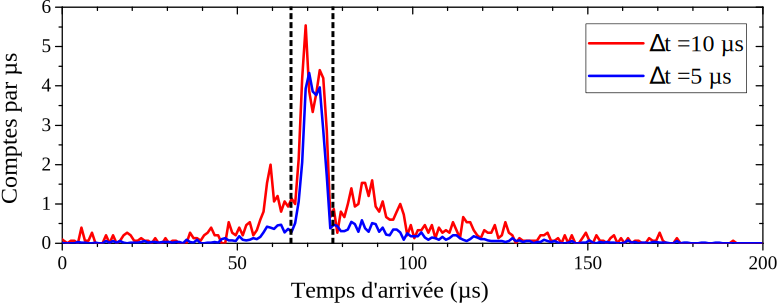
\includegraphics[width=\linewidth]{figures/circulars/arrTimes_50D_inter}
\caption[Signal d'ionisation élargi par interactions du niveau $\mathrm{50D}$]{
Signal d'ionisation élargi par interactions du niveau $\mathrm{50D}$.
La figure présente les signaux d'ionisation obtenus après excitation du niveau de Rydberg $\mathrm{50D}$ à résonance, avec deux temps d'impulsion laser $\Delta \mathrm{t}$ différents, de $\SI{5}{}$ et $\SI{10}{\us}$.
Les traits pointillés verticaux délimitent la fenêtre de détection pour le niveau $\mathrm{50D}$.
}
\label{fig:arrTimes_50D_inter}
\end{figure}
%
Cet élargissement du signal de détection est un problème dès lors que l'on souhaite détecter sélectivement différents niveaux de Rydberg voisins.
En effet, la sélectivité de la détection dépend de la bonne séparation des signaux d'ionisation de chaque niveau.
Ainsi, si l'un d'eux présente un signal d'ionisation élargi, cela brouille la distinction entre les niveaux.
Cela entraîne aussi une saturation artificielle du nombre d'atomes détectés.
Sur la figure \eqref{fig:arrTimes_50D_inter}, dans la fenêtre de détection délimitée par les traits pointillés, on compte respectivement $\SI{28}{}$ et $\SI{36}{}$ atomes de Rydberg pour les deux durées d'impulsion laser de $\SI{5}{}$ et $\SI{10}{\us}$.
Si l'on étend la fenêtre de détection afin de compter tous les ions qui sont arrivés au channeltron, on en compte respectivement $\SI{47}{}$ et $\SI{90}{}$ pour $\SI{5}{}$ et $\SI{10}{\us}$ d'impulsion laser.
On retrouve un régime linéaire du nombre d'atomes de Rydberg excités en fonction du temps, alors que la détection limitée à la première fenêtre semblait saturée.

Afin d'éviter cet effet, nous avons simplement décidé de travailler à plus faible taux d'excitation.
Cela permet de réduire la densité d'atomes de Rydberg et donc les interactions entre eux.
Pour cela, un signal d'ionisation tel que celui à $\SI{5}{\us}$ d'impulsion laser est tout à fait raisonnable.

		
		\subsubsection*{Les sous-niveaux $m_j$ séparés par effet Stark.}
%		\noindent spectres en champ non-nul -> choix de $m_j$ \\
\noindent Dans l'objectif d'exciter par la suite le sous-niveau $\mathrm{50F},m=2$, il est intéressant de lever la dégénérescence du niveau $\mathrm{50D}_{5/2}$.
Pour cela, nous imposons un champ électrique aux atomes, qui lève la dégénérescence par effet Stark.
La figure \eqref{fig:Stark50D5_2} représente les énergies calculées des sous-niveaux $m_j=1/2,3/2$ et $5/2$ du niveau $\mathrm{50D}_{5/2}$ en fonction du champ électrique.
%
\begin{figure}[!h]
\centering
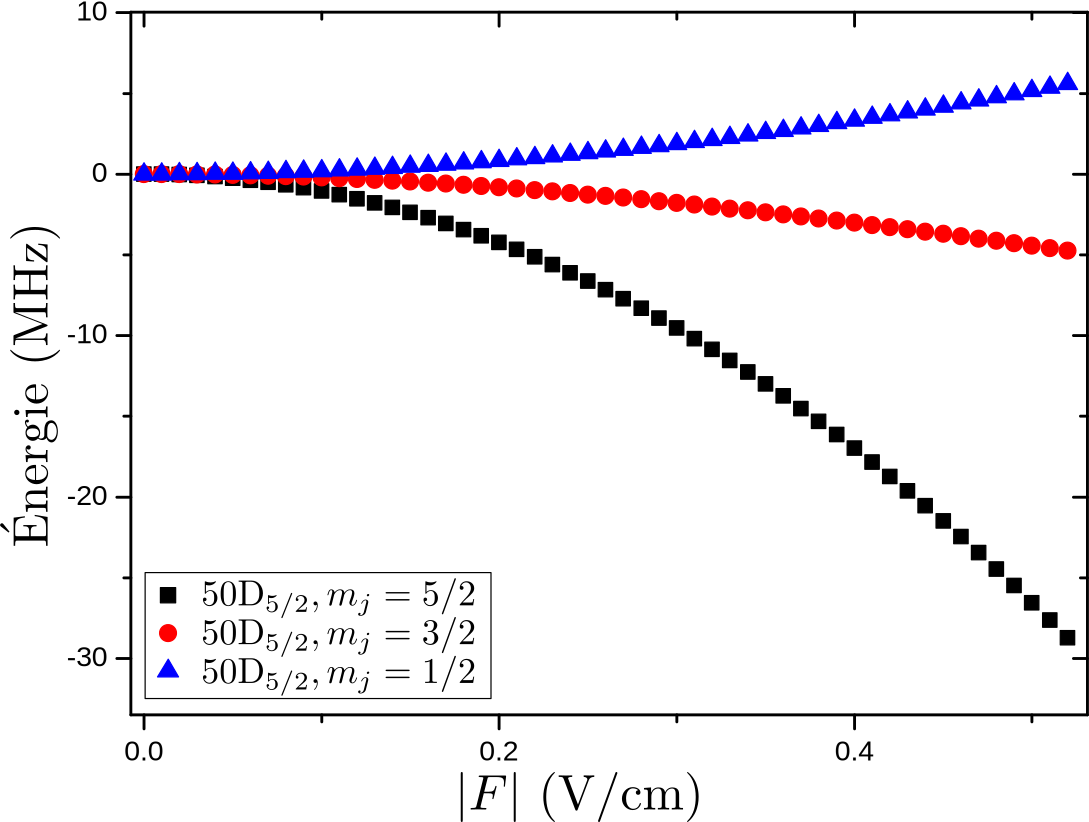
\includegraphics[width=0.7\linewidth]{figures/circulars/Stark50D5_2}
\caption[Diagramme Stark du niveau $\mathrm{50D_{5/2}}$]{
Diagramme Stark du niveau $\mathrm{50D_{5/2}}$.
Le champ électrique $|F|$ sépare le niveau $\mathrm{50D_{5/2}}$ en trois sous-niveau $m_j=1/2,3/2$ et $5/2$.
Le niveau $\mathrm{50D_{3/2}}$ a une énergie trop basse pour être représenté ici.
%Ici, la structure fine domine largement l'effet Stark.
%En champ nul, le niveau $\mathrm{50D_{3/2}}$ a une énergie inférieure de $\SI{93}{\MHz}$ à celle du $\mathrm{50D_{5/2}}$.
%L'effet Stark ne devient dominant par rapport à la structure fine qu'à partir de $\SI{2}{\V/\cm}$ (??).
}
\label{fig:Stark50D5_2}
\end{figure}
%
Tant que le champ électrique reste suffisamment petit, l'effet Stark est traité comme une perturbation agissant au second ordre et les énergies des sous-niveaux en dépendent quadratiquement.
Un ajustement parabolique des données présentées en figure \eqref{fig:Stark50D5_2} donne les coefficients Stark quadratiques présentés en table \eqref{tab:Stark_50D52}.

\begin{table}[!h]
	\centering
	\caption[Effet Stark quadratique des sous-niveaux du $\mathrm{50D}_{5/2}$]{Coefficients d'effet Stark quadratique des des sous-niveaux du $\mathrm{50D}_{5/2}$.
	}
	\label{tab:Stark_50D52}
	\begin{tabular}{c c }
		\toprule\midrule
		Nombre quantique
		& Coefficient Stark quadratique
		\\
		magnétique
		& $A_{\mathrm{50D}_{5/2},m_j}$ en $\si{\MHz \per (\V \per\cm) \squared}$ \\
		\midrule
		$m_j=1/2$
		& \SI[retain-explicit-plus]{+20.78}{} \\
		$m_j=3/2$
		& \SI{-18.52}{} \\
		$m_j=5/2$
		& \SI{-106.16}{} \\
		\midrule
		\bottomrule
 	\end{tabular}
\end{table}

En faisant varier le potentiel appliqué aux électrodes d'ionisation, nous avons été en mesure de résoudre les trois sous-niveaux $m_j$ du niveau $\mathrm{50D}_{5/2}$ par excitation laser.
Un spectre laser enregistré sous un champ électrique de $\SI{0.17}{\V/cm}$ est présenté en figure \eqref{fig:spectre_laser_champ}.
%
\begin{figure}[!h]
\centering
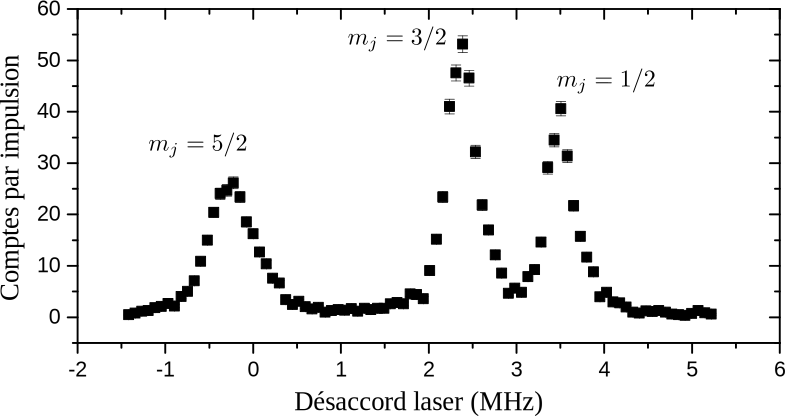
\includegraphics[width=0.85\linewidth]{figures/circulars/spectre_laser_champ}
\caption[Spectre laser de la transition $\mathrm{5S\rightarrow 50D}$ en champ non nul]{
Spectre laser de la transition $\mathrm{5S\rightarrow 50D}$ en champ non nul.
Le champ électrique vaut $|F| = \SI{0.17}{\V/\cm}$.
Les trois sous-niveaux $m_j$ sont bien résolus.
La largeur supérieure du sous-niveau $m_j=5/2$ est attribué à un élargissement Stark inhomogène en raison de sa plus grande sensibilité (cf table \eqref{tab:Stark_50D52}).
}
\label{fig:spectre_laser_champ}
\end{figure}
%
Nous pouvons ainsi choisir quel sous-niveau $\mathrm{50D}_{5/2},m_j$ nous excitons en ajustant la fréquence du laser bleu.

Il aurait été possible de choisir quel sous-niveau exciter en ajustant la polarisation des lasers.
Malheureusement, le dispositif optique actuel ne permet pas de choisir la polarisation du faisceau laser rouge, celui-ci étant superposé sur un cube polariseur à l'un des faisceaux de piégeage magnéto-optique.
De plus, le champ électrique que nous imposons définit l'axe de quantification selon $Oy$.
Dans cette géométrie, il est impossible de distinguer les polarisations circulaires $\sigma^+$ et $\sigma^-$ pour des faisceaux laser se propageant selon l'axe $Ox$.
%Un réaménagement de l'optique d'excitation, associé à un axe de quantification défini selon l'axe $Ox$ pourrait permettre d'adresser les différents sous-niveaux $m_j$
Plutôt que d'effectuer un réaménagement de l'optique d'excitation et des rotations de l'axe de quantification, nous avons préféré nous limiter à lever la dégénérescence par un champ électrique selon $Oy$.

Ce choix mène à une réduction du nombre d'atomes de Rydberg excités, en particulier pour le sous-niveau $m_j=5/2$ qui subit un élargissement Stark inhomogène.
Cette moindre efficacité de l'excitation n'est cependant pas un problème car nous pouvons augmenter les puissances des faisceaux laser ainsi que la durée d'impulsion afin de la compenser.



\newpage
	\subsection{La transition microonde $\mathrm{50D \rightarrow 50F}$}
\noindent %fréquence de la transition, arrTimes, spectre en champ nul, Rabi ?? \\
Après avoir excité le niveau de Rydberg $\mathrm{50D}_{5/2}$, nous souhaitons transférer les atomes dans le sous-niveau $\mathrm{50F},m=2$.
Intéressons-nous en premier lieu à la transition microonde $\mathrm{50D_{5/2} \rightarrow 50F}$ en champ électrique nul.
Cette transition se fait à la fréquence
\begin{equation}
\label{eq:freq_50D50F}
\nu_{\mathrm{50D_{5/2}\rightarrow50F}}(F=0)% = \frac{1}{h}\left( E_{50D_{5/2}}(F=0) - E_{50F}(F=0) \right)
= \SI{72.9594}{\GHz}
\end{equation}

Cette transition est dans le domaine microonde.
Afin de générer le champ microonde nécessaire, nous utilisons une source Anritsu MG3692C, générant un signal oscillant à $\SI{18}{\GHz}$, dont la fréquence peut être balayée.
Ce signal est amené par câble à un quadrupleur actif Militech AMC-15-RFH00.
Le signal à $\SI{72}{\GHz}$ généré par ce quadrupleur est transporté par un guide d'onde circulaire de diamètre $\SI{5.6}{\mm}$ jusqu'à un cornet microonde situé devant le hublot de face à l'extérieur du cryostat.

La détection par ionisation permet de distinguer les deux niveaux de Rydberg.
La figure \eqref{fig:arrTimes_50D50F} représente les signaux d'ionisation obtenus avec et sans impulsion microonde sur la transition $\mathrm{50D_{5/2} \rightarrow 50F}$.
%
\begin{figure}[!h]
\centering
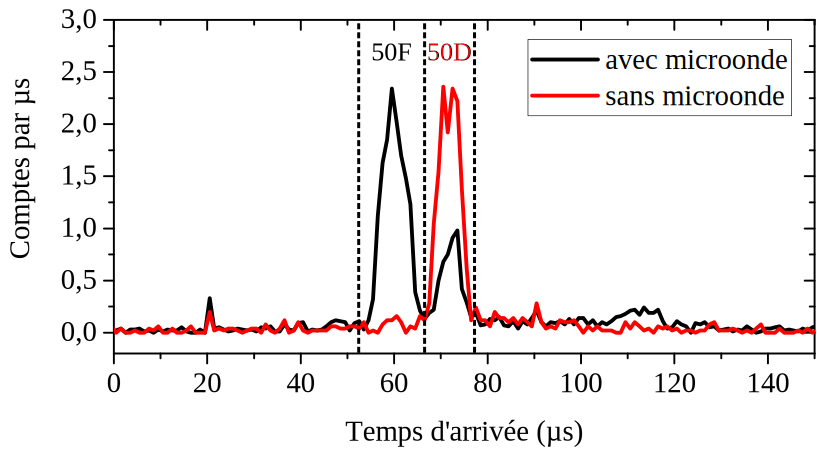
\includegraphics[width=0.85\linewidth]{figures/circulars/arrTimes_50D50F}
\caption[Signal d'ionisation $\mathrm{50D\rightarrow 50F}$]{
Signal d'ionisation $\mathrm{50D\rightarrow 50F}$.
La courbe rouge présente le signal d'ionisation obtenu après excitation laser du niveau $\mathrm{50D}$.
La courbe noire présente le signal d'ionisation obtenu après excitation laser du niveau $\mathrm{50D}$ et application d'une impulsion microonde optimisée sur la transition $\mathrm{50D \rightarrow 50F}$.
Les traits pointillés représentent les limites des fenêtres de détection.
}
\label{fig:arrTimes_50D50F}
\end{figure}
%
La séparation entre les signaux d'ionisation de chaque niveau est suffisante pour définir des fenêtres de détection pour chacun.

La difficulté principale de la transition $\mathrm{50D} \rightarrow\mathrm{50F}$ réside dans la très grande sensibilité Stark du niveau $\mathrm{50F}$.
Celui-ci présente un coefficient Stark quadratique compris entre $\SI{-4}{}$ et $\SI{-8}{\GHz/(\V/\cm)\squared}$.
En raison de cette sensibilité au champ électrique, bien plus grande que celle du $\mathrm{50D}$, la transition vers le niveau $\mathrm{50F}$ subit un élargissement Stark inhomogène très important.

Il nous a donc fallu effectuer une optimisation fine des potentiels appliqués aux électrodes d'ionisation afin d'obtenir un champ nul selon la direction $y$, ainsi qu'aux quatre électrodes RF, afin d'obtenir un champ nul selon les directions $x$ et $z$.
L'optimisation du seul champ selon $y$ ne nous permet d'obtenir une largeur spectrale de l'ordre de $\SI{6}{\MHz}$.
L'optimisation des champs selon $x$ et $z$ nous a ensuite permis de réduire cette largeur à moins de $\SI{1}{\MHz}$, en ajustant la durée d'impulsion et la puissance du signal microonde.
Le spectre ainsi obtenu, pour une durée d'impulsion $\Delta t _{mo} = \SI{4}{\us}$ et une puissance microonde $P_{\text{Anritsu}} = \SI{5}{\dBm}$ à la sortie de la source Anritsu, est représenté en figure \eqref{fig:spectres_mw_champnul}.
%
\begin{figure}[!h]
\centering
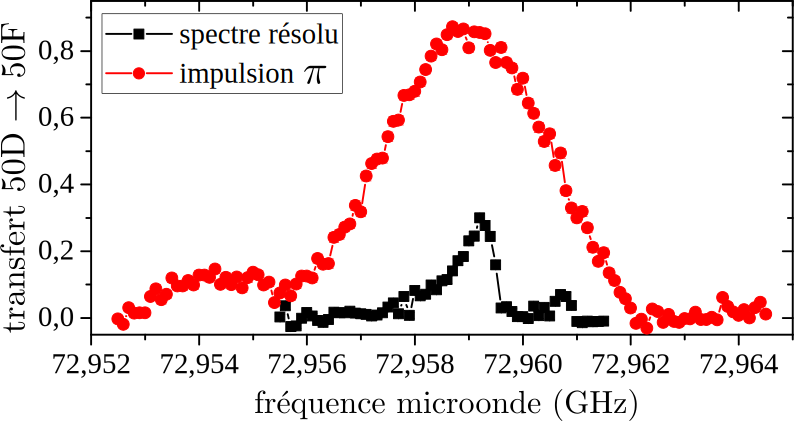
\includegraphics[width=0.85\linewidth]{figures/circulars/spectres_mw_champnul}
\caption[Spectre microonde de la transition $\mathrm{50D\rightarrow 50F}$ en champ nul]{
Spectre microonde de la transition $\mathrm{50D\rightarrow 50F}$ en champ nul.
}
\label{fig:spectres_mw_champnul}
\end{figure}
%
À partir de ce spectre résolu, nous avons pu mesurer des oscillations de Rabi sur cette transition, en suivant le taux de transfert $\mathrm{50D \rightarrow 50F}$ en fonction de la durée de l'impulsion microonde, pour différentes puissances.
Cela nous a permis de définir une impulsion $\pi$ à grande fréquence de Rabi permettant de transférer jusqu'à $\SI{90}{\percent}$ des atomes vers le niveau $\mathrm{50F}$.
Le spectre ainsi obtenu, pour $\Delta t_{mo} = \SI{0.3}{\us}$ et $P_{\text{Anritsu}} = \SI{13}{\dBm}$, est représenté en figure \eqref{fig:spectres_mw_champnul}.

\subsubsection*{Les sous-niveaux $m$ séparés par effet Stark}
%	\noindent en champ non-nul -> choix de $m_l$ et problème d'élargissement Stark, optimisation des champs
\noindent \`A partir des spectres optimisés en champ électrique nul, nous avons progressivement augmenté le champ électrique selon la direction $y$ afin de lever la dégénérescence des sous-niveau $m$ du $\mathrm{50F}$.
Le couplage fin pour le niveau $\mathrm{50F}$ est de l'ordre de $\SI{1.3}{\MHz}$.
Ce couplage est dominé par l'effet Stark dès lors que le champ électrique dépasse $\SI{0.02}{\V/\cm}$.
Pour cette raison, bien que nous continuions à considérer les sous-niveaux $m_j$ du niveau $\mathrm{50D}_{5/2}$, la base adaptée pour le niveau $\mathrm{50F}$ est celle des sous-niveaux $m$.
Le schéma de niveaux de la transition $\mathrm{50D}_{5/2}\rightarrow\mathrm{50F}$ est présenté en figure \eqref{fig:levels_50D50F}.
La figure \eqref{fig:Stark50F} représente les énergies calculées des sous-niveaux du $\mathrm{50F}$ en fonction du champ électrique.
Un ajustement parabolique donne les coefficients Stark quadratiques présentés en table \eqref{tab:Stark_50F}.

\begin{figure}[!h]
\centering
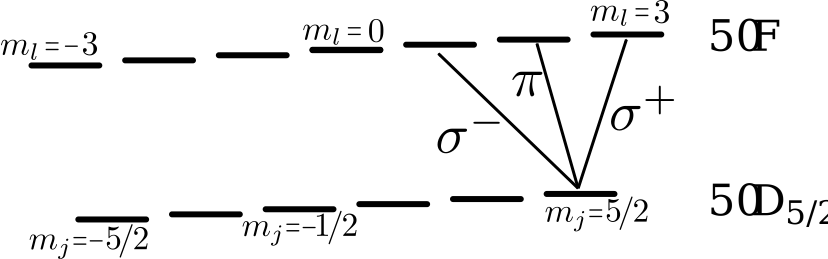
\includegraphics[width=0.7\linewidth]{figures/circulars/levels_50D50F}
\caption[Schéma de niveaux de la transition $\mathrm{50D\rightarrow 50F}$]{
Schéma de niveaux de la transition $\mathrm{50D_{5/2}\rightarrow 50F}$.
La structure fine est négligeable pour le $\mathrm{50F}$, qui se divise en sous-niveaux $m_l$.
}
\label{fig:levels_50D50F}
\end{figure}
%
\begin{figure}[!h]
\centering
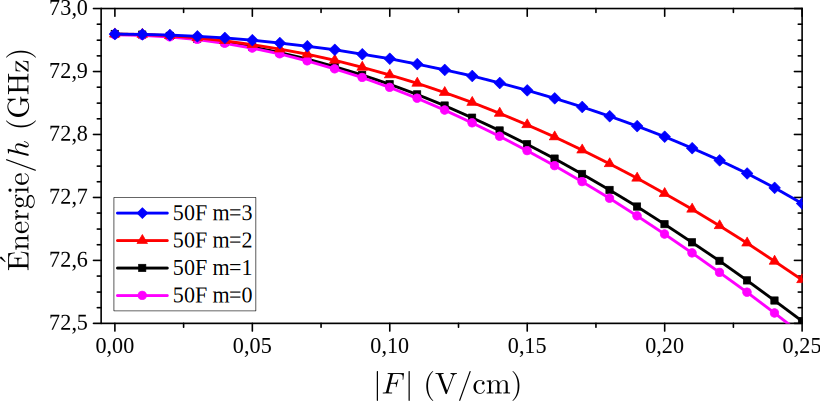
\includegraphics[width=\linewidth]{figures/circulars/Stark50F}
\caption[Diagramme Stark d'énergie du niveau $\mathrm{50F}$]{
Diagramme Stark d'énergie du niveau $\mathrm{50F}$.
Les traits pleins sont des guides visuels entre les points calculés.
Le champ électrique $|F|$ sépare le niveau $\mathrm{50F}$ en trois sous-niveau $m=1,2$ et $3$.
La structure fine est négligeable.
L'origine des énergies est définie par le niveau $\mathrm{50D}_{5/2}$ en champ nul.
}
\label{fig:Stark50F}
\end{figure}
%
\begin{table}[!h]
	\centering
	\caption[Effet Stark quadratique des sous-niveaux du $\mathrm{50F}$]{Coefficients d'effet Stark quadratique des des sous-niveaux du $\mathrm{50F}$.
	}
	\label{tab:Stark_50F}
	\begin{tabular}{c c }
		\toprule\midrule
		Nombre quantique
		& Coefficient Stark quadratique
		\\
		magnétique
		& $A_{\mathrm{50D}_{5/2},m_j}$ en $\si{\MHz \per (\V \per\cm) \squared}$ \\
		\midrule
		$m=0$
		& \SI{-8145.4}{} \\
		$m=1$
		& \SI{-7680.0}{} \\
		$m=2$
		& \SI{-6332.7}{} \\
		$m=3$
		& \SI{-3945.9}{} \\
		\midrule
		\bottomrule
 	\end{tabular}
\end{table}
%

La figure \eqref{fig:spectre_mw_champ} présente un spectre de la transition $\mathrm{50D}_{5/2},m_j=5/2 \rightarrow \mathrm{50F}$ sous un champ électrique de $\SI{0.19}{\V/\cm}$.
%
\begin{figure}[!h]
\centering
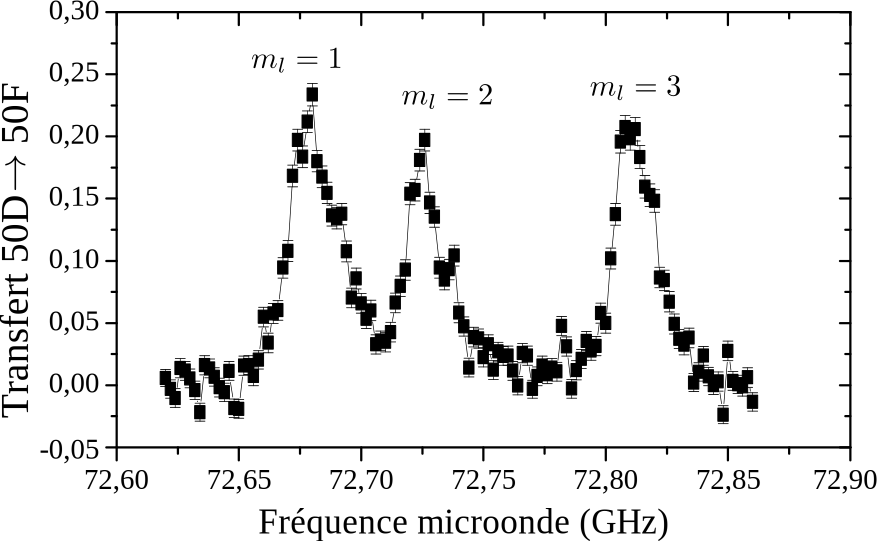
\includegraphics[width=0.85\linewidth]{figures/circulars/spectre_mw_champ}
\caption[Spectre microonde de la transition $\mathrm{50D\rightarrow 50F}$ en champ non nul]{
Spectre microonde de la transition $\mathrm{50D\rightarrow 50F}$ en champ non nul.
Le champ électrique vaut $|F| = \SI{0.19}{\V/\cm}$.
Les trois sous-niveaux $m=1,2,3$ sont résolus malgré l'élargissement Stark important.}
\label{fig:spectre_mw_champ}
\end{figure}
%
L'élargissement Stark inhomogène est tel que nous n'avons pu obtenir des taux de transferts supérieurs à $\SI{25}{\percent}$.
Le facteur limitant ici est la puissance microonde disponible.
En effet, le quadrupleur amplifié Militech AMC-15-RFH00 admet une puissance nominale de $\SI[retain-explicit-plus]{+3}{\dBm}$ en entrée et nous ne disposons pas d'amplificateur fonctionnant aux fréquences utilisées.
De plus, le champ microonde est émis à l'extérieur du cryostat.
L'installation d'un guide d'onde débouchant à l'intérieur du cryostat au plus près des atomes permettrait d'augmenter significativement la puissance microonde disponible.

\subsubsection*{Les paramètres choisis}
\noindent En optimisant les conditions d'excitation, nous avons pu porter à $\SI{12}{}$ le nombre d'atomes excités après chaque impulsion laser dans le sous-niveau $\mathrm{50F},m=2$, sous un champ électrique de $\SI{0.19}{\V/cm}$.
Une valeur de champ électrique plus petite permettrait d'en exciter beaucoup plus, mais nous ne pourrions plus résoudre les différents sous-niveaux $m$ du niveau $\mathrm{50F}$.

De façon surprenante, l'excitation du $\mathrm{50F}$ depuis le sous-niveau $\mathrm{50D}_{5/2}, m_j = 3/2$ donne un spectre plus large et donc moins résolu.
Nous attribuons cela à l'élargissement Stark inhomogène plus important subi par le sous-niveau $\mathrm{50D}_{5/2}, m_j = 5/2$.
En raison de celui-ci, la fréquence laser effectue une sélection spatiale des atomes excités de façon résonante depuis le niveau fondamental vers le $\mathrm{50D}_{5/2}, m_j = 5/2$.
Le nuage d'atomes de Rydberg $\mathrm{50D}$ est par conséquent moins étendu spatialement, limitant ainsi l'élargissement Stark inhomogène de la transition $\mathrm{50D}\rightarrow\mathrm{50F}$.

%\newpage
	\subsection{Le passage adiabatique $m=2\rightarrow m=n-1$}
%		\noindent passage adiabatique : séquence type
\noindent \`A partir du sous-niveau $\mathrm{50F},m=2$, nous pouvons effectuer un passage adiabatique radio-fréquence vers le niveau circulaire $\mathrm{50C}$.
Pour cela, il nous faut augmenter fortement le champ électrique, de façon rendre la transition depuis le sous-niveau $\mathrm{50F},m=2$ vers le reste de la multiplicité résonante avec les transitions $\sigma^+$ à l'intérieur de cette même multiplicité, comme nous l'avons expliqué en \ref{subsec:adiab_Qdefect}.
Après cette étape de \og branchement Stark \fg{}, des tensions oscillantes à $\nu_{RF} = \SI{230}{\MHz}$ sont appliquées aux quatre électrodes RF, générant le champ radio-fréquence nécessaire au passage adiabatique.
La séquence d'excitation correspondante est représentée en figure \eqref{fig:seq_circul}.

\begin{figure}[!h]
\centering
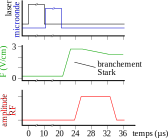
\includegraphics[width=.7\linewidth]{figures/circulars/seq_circul}
\caption[Séquence d'excitation des atomes de Rydberg circulaires]{
Séquence d'excitation des atomes de Rydberg circulaires.
Le champ électrique initial est de $\SI{0.2}{\V/\cm}$.
L'impulsion laser de $\SI{10}{\us}$ excite les atomes du niveau fondamental vers le niveau $\mathrm{50D}_{5/2},m_j=5/2$.
L'impulsion microonde de $\SI{6}{\us}$ transfère $\SI{20}{\percent}$ des atomes de Rydberg vers le niveau $\mathrm{50F},m=2$.
Le module du champ électrique est augmenté jusqu'à $\SI{2.7}{\V/\cm}$ lors du \og branchement Stark \fg{} puis la radio-fréquence est allumée pour le passage adiabatique.
Pendant celui-ci, le module du champ électrique est diminué jusqu'à $\SI{2.3}{\V/\cm}$ en $\SI{2}{\us}$.
Enfin, la radio-fréquence est éteinte.
}
\label{fig:seq_circul}
\end{figure}

\subsubsection*{Le dispositif radio-fréquence}
\noindent Afin de réaliser le passage adiabatique, nous devons appliquer aux quatre électrodes RF des tensions oscillantes dont les phases relatives et les amplitudes sont bien contrôlées.
Pour cela, nous avons mis au point un dispositif d'émission et de contrôle radio-fréquence, inspiré de celui mis au point dans notre laboratoire par Sébastien Gleyzes, Adrien Signoles et Adrien Facon \cite{PHD_SIGNOLES,PHD_FACON}.
Ce dispositif est représenté en figure \eqref{fig:RF_control}

\begin{sidewaysfigure}
\centering
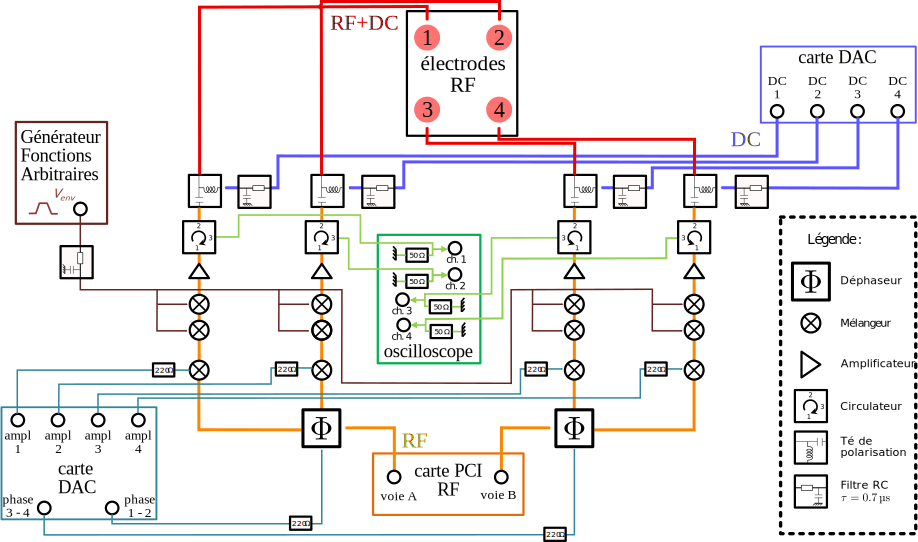
\includegraphics[width=\linewidth]{figures/circulars/RF_control}
\caption[Dispositif de contrôle radio-fréquence]
{Dispositif de contrôle radio-fréquence pour la circularisation des atomes de Rydberg}
\label{fig:RF_control}
\end{sidewaysfigure}

Une carte PCI Acquitek Synth-3000 génère, sur chacune de ses deux voies de sortie, un signal électrique oscillant à $\SI{230}{\MHz}$.
La phase relative entre ces deux voies $A$ et $B$ est contrôlée par le logiciel de contrôle de la carte PCI.
Le signal généré par chacune de ces deux voies est envoyé vers un déphaseur PULSAR ST-H85-444A, qui sépare le signal sur deux voies avec une phase relative contrôlée par une tension continue.
Nous disposons ainsi de quatre voies radio-fréquence dont les phases relatives sont contrôlées.

Chacune de ces quatre voies suit ensuite parallèlement le même chemin.
Le signal est envoyé sur un mélangeur PULSAR X2L-06-411 alimenté par une tension continue, et est ainsi modulé en amplitude.
Ensuite, deux mélangeurs PULSAR X2L-06-411 successifs servent d'interrupteur pour bloquer ou laisser passer le signal radio-fréquence.
Le signal est ensuite amplifié par un amplificateur WENTEQ ABP0100-10-3029, puis passe dans un circulateur HYTEM 09-02-57, qui protège l'amplificateur en redirigeant le signal réfléchi vers une terminaison $\SI{50}{\ohm}$ ou vers une voie d'oscilloscope.
Enfin, le signal est superposé à une tension constante dans un té de polarisation PULSAR BT-20-411.
Cette tension constante sert au contrôle des champs statiques au niveau des atomes selon les directions $x$ et $z$.
La sortie du té de polarisation est ensuite câblée à travers le cryostat jusqu'à l'électrode RF correspondant à la voie choisie.

Toutes les tensions continues sont générées par des cartes DAC contrôlées par ordinateur.
Les tensions des deux déphaseurs et les tensions contrôlant l'amplitude radio-fréquence sur chaque voie passent par des résistances de charge de $\SI{220}{\ohm}$.
Les tensions envoyées directement aux électrodes sont passées par un filtre RC passe-bas constitué d'une résistance de $\SI{47}{\ohm}$ et d'un condensateur de $\SI{15}{\nano\farad}$.
La constante de temps de ce filtre est de $\SI{0.7}{\us}$ et permet de limiter le bruit haute fréquence au niveau des électrodes à moins de $\SI{5}{\milli\volt}$ pic à pic.

La tension $V_{env}$ alimentant les mélangeurs \og interrupteurs \fg{} est générée par un générateur de fonctions arbitraires qui nous permet de mettre en forme l'impulsion RF et de contrôler la vitesse de l'allumage et de l'extinction du champ radio-fréquence.
Cette tension passe par une filtre RC, identique à celui utilisé pour les tensions continues appliquées aux électrodes.


\subsubsection*{Procédure initiale d'ajustement des amplitudes et phases RF}
%		\noindent arrTimes avec différentes puissances RF + la procédure d'optimisation
\noindent La difficulté technique du passage adiabatique réside dans le contrôle des amplitudes et des phases du signal envoyé à chaque électrode afin de produire un champ polarisé $\sigma^+$ le plus pur possible.
Nous avons utilisé une procédure d'optimisation mise au point par Sébastien Gleyzes, Adrien Signoles et Adrien Facon.
L'objectif initial de cette optimisation est de progresser sur l'échelle de niveaux du passage adiabatique.
Comme nous l'avons déjà mentionné, les niveaux à haut moment cinétique ont un seuil d'ionisation plus élevé que les niveaux à bas moment cinétique.
En particulier, le seuil d'ionisation croît à mesure que les atomes progressent sur l'échelle du passage adiabatique en direction du niveau circulaire.
Le signal d'ionisation des atomes de Rydberg permet ainsi d'estimer l'efficacité du passage adiabatique.
%
%%
%\begin{figure}[h]
%\centering
%arr Times à différentes étapes de l'optimisation
%29 aout cahier 20 pp.57-65
%\caption[Signaux d'ionisation lors de l'optimisation RF]{
%Signaux d'ionisation lors de l'optimisation RF
%}
%\label{fig:arrTimes_optim_RF}
%\end{figure}
%%
%La figure \ref{fig:arrTimes_optim_RF} présente des signaux d'ionisation à différentes étapes de la procédure d'optimisation passage adiabatique, présentée ci-dessous :
La procédure d'optimisation est détaillée ci-dessous :
%
\begin{enumerate}
\item \label{item:RFoptim1} Régler la tension de commande $V_{ampl~1}$ de la puissance envoyée à l'électrode $1$ seulement, toutes les autres voies étant éteintes, de façon à pousser vers les plus hauts champs électriques le signal d'ionisation.
\item Effectuer le même réglage sur les électrodes $2,3$ et $4$ chacune à son tour.
\item Avec les électrodes $1$ et $2$ à $V_{ampl~1,2}$ respectivement, ajuster la tension de commande $V_{\phi~1-2}$ qui alimente règle la phase relative entre les voies $1$ et $2$, de façon à repousser vers les plus hauts champs et à affiner le pic d'ionisation.
\item Effectuer de la même façon le réglage de $V_{\phi~3-4}$, avec les électrodes $3$ et $4$ seulement.
\item Avec les quatre électrodes allumées, ajuster la phase $\phi_{A-B}$ pour obtenir une interférence constructive entre le champ $\sigma^+$ créé par la paire $1-2$ et le champ $\sigma^+$ créé par la paire $3-4$.
\item Régler la tension $V_{env}$ qui crée l'enveloppe de l'impulsion radio-fréquence pour leq autres électrodes.
\item Recommencer en \ref{item:RFoptim1}.
\end{enumerate}

%
\begin{figure}[!h]
\centering
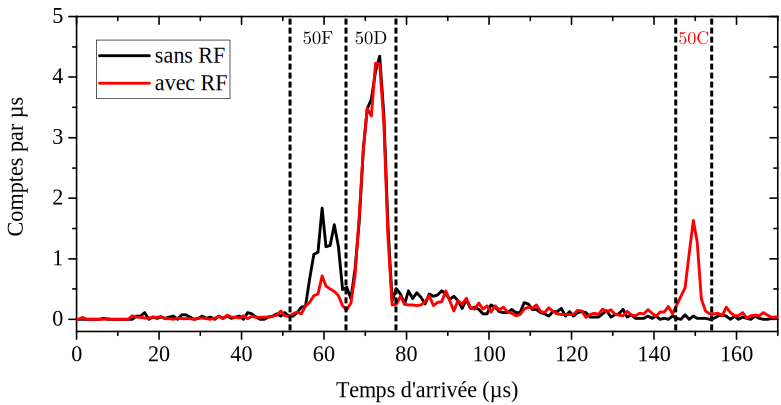
\includegraphics[width=0.85\linewidth]{figures/circulars/arrTimes_with-without_RF}
\caption[Signaux d'ionisation des atomes circulaires]{
Signaux d'ionisation à l'issue de la procédure d'optimisation.
La courbe rouge présente le signal d'ionisation obtenu après excitation laser, impulsion microonde $\mathrm{50D \rightarrow 50F}$ et passage adiabatique radiofréquence.
La courbe noire présente le signal d'ionisation obtenu en éteignant le champ radio-fréquence pendant le passage adiabatique.
Les traits pointillés représentent les limites des fenêtres de détection.
}
\label{fig:arrTimes_with-without_RF}
\end{figure}
%
\`A l'issue de l'optimisation RF, nous obtenons le signal d'ionisation présenté en figure \eqref{fig:arrTimes_with-without_RF}, qui montre un pic très clair $\SI{150}{\us}$ après le début de la rampe.
Ce pic est \textit{a priori} dû à des atomes de Rydberg circulaires, mais la détection par ionisation n'est pas assez résolue pour les distinguer d'atomes dans le niveaux elliptiques proches du circulaire.
%Le nombre d'atomes circulaires excités ici est de $\SI{5}{}\pm\SI{1}{}$ après chaque impulsion laser.

%\newpage
\section{Spectroscopie microonde des atomes de Rydberg circulaires}
\noindent La caractérisation précise des atomes de Rydberg circulaires se fait par spectroscopie microonde des transitions vers les niveaux circulaires des multiplicités voisines.
%
Le schéma de niveaux pour les transitions du $\mathrm{50C}$ vers les niveaux $\mathrm{49C}$ et $\mathrm{51C}$ est présenté en figure \eqref{fig:levels_49-50-51C}.
%	\subsection{Transitions microonde vers les niveaux voisins}
%\noindent schéma de niveaux 49-50-51c, Stark différentiel et arrTimes
\begin{figure}[h]
\centering
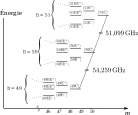
\includegraphics[width=.7\linewidth]{figures/circulars/levels_49-50-51C}
\caption[Schéma de niveaux pour la spectroscopie microonde des Rydberg circulaires]{
Schéma de niveaux pour la spectroscopie microonde des Rydberg circulaires.
}
\label{fig:levels_49-50-51C}
\end{figure}
%

En champ électrique nul, toutes les transitions depuis la multiplicité $n$ vers la multiplicité $n-1$ ont la même fréquence.
Grâce à l'effet Stark, qui lève la dégénérescence entre les niveaux d'une même multiplicité, ces transitions deviennent discernables.
Les coefficients Stark linéaires et quadratiques pour les transitions $50-49$ et $50-51$ sont résumés en table \eqref{tab:Stark_49-50-51C}.		
%
\begin{table}[!h]
	\centering
	\caption[Transitions microonde depuis le niveau $\mathrm{50C}$ et effet Stark différentiel]{
	Transitions microonde depuis le niveau $\mathrm{50C}$ et effet Stark différentiel
	}
	\label{tab:Stark_49-50-51C}
	\begin{tabular}{cccc}
		\toprule\midrule
		Transition
		& Fréq. en champ nul
		& Coef. Stark linéaire
		& Coef. Stark quadratique
		\\
		atomique
		& $\si{\GHz}$
		& $\si{\MHz \per (\V \per\cm)}$
		& $\si{\MHz \per (\V \per\cm) \squared}$ \\
		\midrule
		$\mathrm{50C \rightarrow 51C}$
		& \SI{51.0991}{}
		& \SI{0}{}
		& \SI{-0.254}{} \\
		$\mathrm{50E^+ \rightarrow 51E^+}$
		& \SI{51.0991}{}
		& \SI[retain-explicit-plus]{+1.92}{}
		& \SI{-0.263}{} \\
		$\mathrm{50E^- \rightarrow 51E^-}$
		& \SI{51.0991}{}
		& \SI[retain-explicit-plus]{-1.92}{}
		& \SI{-0.263}{} \\
		$\mathrm{50EE^+ \rightarrow 51EE^+}$
		& \SI{51.0991}{}
		& \SI[retain-explicit-plus]{+3.84}{}
		& \SI{-0.272}{} \\
		$\mathrm{50EE^- \rightarrow 51EE^-}$
		& \SI{51.0991}{}
		& \SI[retain-explicit-plus]{-3.84}{}
		& \SI{-0.273}{} \\
		\midrule
		$\mathrm{50C \rightarrow 49C}$
		& \SI{54.2594}{}
		& \SI{0}{}
		& \SI{-0.230}{} \\
		$\mathrm{50E^+ \rightarrow 49E^+}$
		& \SI{54.2594}{}
		& \SI[retain-explicit-plus]{+1.92}{}
		& \SI{-0.239}{} \\
		$\mathrm{50E^- \rightarrow 49E^-}$
		& \SI{54.2594}{}
		& \SI[retain-explicit-plus]{-1.92}{}
		& \SI{-0.239}{} \\
		$\mathrm{50EE^+ \rightarrow 49EE^+}$
		& \SI{54.2594}{}
		& \SI[retain-explicit-plus]{+3.84}{}
		& \SI{-0.247}{} \\
		$\mathrm{50EE^- \rightarrow 49EE^-}$
		& \SI{54.2594}{}
		& \SI[retain-explicit-plus]{-3.84}{}
		& \SI{-0.247}{} \\
		\midrule
		\bottomrule
 	\end{tabular}
\end{table}
%
La spectroscopie de l'une de ces deux transitions en champ électrique non nul nous permettra ainsi de repérer les atomes dans les niveaux elliptiques proches du $\mathrm{50C}$.
Une optimisation fine des amplitudes et phases radio-fréquence lors du passage adiabatique permettra de les éliminer.

	\subsubsection*{Signaux d'ionisation et limite sur les tensions d'ionisation}
%	\noindent on peut pas dépasser $\sim 450-470V$ à cause des optocoupleurs -> limite déjà pour les 50C et on perd trop de signal pour les 49C -> choix du 51c pour la spectro, mais ça permet pas de faire une purif ..
\noindent La figure \eqref{fig:arrTimes_49-50-51C} présente les signaux d'ionisation des atomes de Rydberg après circularisation vers le niveau $\mathrm{50C}$, et après circularisation puis transition du $\mathrm{50C}$ vers les niveaux $\mathrm{49C}$ et $\mathrm{51C}$.
%
\begin{figure}[h]
\centering
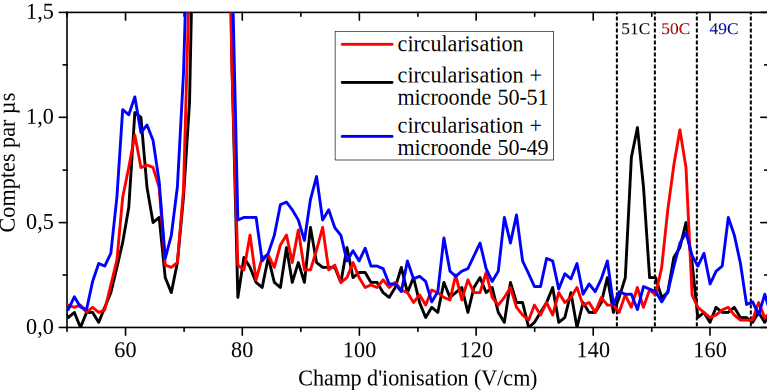
\includegraphics[width=.85\linewidth]{figures/circulars/arrTimes_49-50-51C}
%arrTimes 008 et 009 du 1er septembre (cahier 20 p.120) pour le 51C
%arrTimes 023 et 024 du 31 aout (cahier 20 p.98) pour le 49C
\caption[Signaux d'ionisation pour la spectroscopie microonde des niveaux circulaires]{
Signaux d'ionisation pour la spectroscopie microonde des niveaux circulaires.
À gauche, les pics des niveaux $\mathrm{50D}$ et $\mathrm{50F}$ sont les mêmes pour les trois courbes.
À droite, le pic rouge correspond aux atomes dans le niveau $\mathrm{50C}$ après circularisation.
Le pic noir apparaît après application d'une impulsion microonde correspondant à la transition $\mathrm{50C}\rightarrow \mathrm{51C}$ alors que le pic bleu apparaît après application d'une impulsion microonde correspondant à la transition $\mathrm{50C}\rightarrow \mathrm{49C}$.
Les traits pointillés représentent les limites des fenêtres de détection.
}
\label{fig:arrTimes_49-50-51C}
\end{figure}
%
Comme attendu, le niveau $\mathrm{51C}$ s'ionise avant le $\mathrm{50C}$, donc à champ plus faible, et le $\mathrm{49C}$ s'ionise après le $\mathrm{50C}$, donc à champ plus fort.

%La rampe de potentiel que nous appliquons aux électrodes d'ionisation est d'une durée de $\SI{170}{\us}$.
La rampe de potentiel que nous appliquons aux électrodes d'ionisation est programmée de façon à ce que le potentiel atteigne $\SI{-500}{\V}$, ce qui est la limite de fonctionnement de l'amplificateur.
Malheureusement, les optocoupleurs MOC8204M utilisés dans le circuit de commutation ne bloquent pas les tensions aussi hautes.
Lorsque la tension à leurs bornes atteint $\SI{-465}{\V}$ environ, les optocoupleurs qui servent à bloquer la voie basse tension du circuit de commutation deviennent passants.
L'excès de tension est alors automatiquement mis à la masse par la sortie du générateur "Stark" basse tension.
On ne peut ainsi imposer un potentiel supérieur en valeur absolue à $\SI{465}{\V}$ aux électrodes d'ionisation.
Or le pic d'ionisation du niveau $\mathrm{49C}$ se situe tout à la fin de la rampe d'ionisation, dont la durée totale est de $\SI{160}{\us}$.
L'ionisation du $\mathrm{49C}$ a donc lieu alors que le potentiel d'ionisation est proche de la saturation et nous risquons de perdre significativement en efficacité de détection pour ce niveau.
Nous privilégierons pour cette raison la spectroscopie de la transition $\mathrm{50C \rightarrow 51C}$.

	\subsection{Spectres microonde et optimisation fine de la RF}

\noindent Les impulsions microonde pour la spectroscopie des niveaux circulaires ont été générées par la source Anritsu MG3692C que nous utilisions pour adresser la transition $\mathrm{50D \rightarrow 50F}$.
Nous avons ajouté une source microonde Anapico APSYN420 pour générer le champ microonde nécessaire à cette première transition, libérant ainsi la source Anritsu pour la spectroscopie.
Les premiers spectres  de la transition $\mathrm{50C-51C}$ sont représentés en figure \eqref{fig:spectre_50C51C_nofield-field} pour deux valeurs de champ électrique : $\SI{0.19}{}$ et $\SI{0.9}{\V/\cm}$.
%
\begin{figure}[h]
\centering
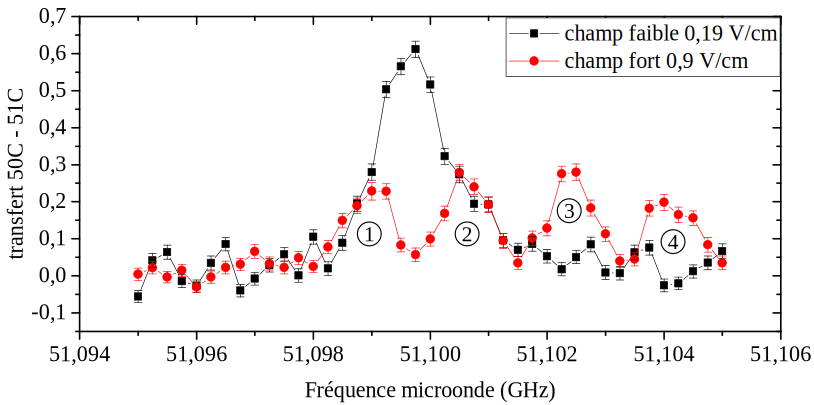
\includegraphics[width=.85\linewidth]{figures/circulars/spectre_50C51C_nofield-field}
%Ryd0068 et 0070 du 31 aout (cahier 20 p.108)
\caption[Premiers spectres microonde 50C-51C]{
%$P_Anritsu = -1.5 dBm	\Delta t = 0.9 \mus$
Premiers spectres microonde 50C-51C, pour deux valeurs de champs électrique :
$\SI{0.19}{\V/\cm}$ (courbe noire) et $\SI{0.9}{\V/\cm}$ (courbe rouge).
Les deux spectres sont enregistrés avec une puissance microonde $P_{\text{Anritsu}} = \SI{-1.5}{\dBm}$ à la sortie de la source et une durée d'impulsion $\Delta t _{mo} = \SI{0.9}{\us}$, correspondant à une impulsion $\pi$.
Le spectre en champ faible présente un seul pic proche de la fréquence attendue de $\SI{51.099}{\GHz}$, limité par transformée de Fourier en raison de la durée d'impulsion.
Le spectre en champ \og fort \fg{} montre quatre pics, indicatifs d'une population importante dans les niveaux elliptiques de la diagonale supérieure.
% situés aux fréquences des transitions 
%$\mathrm{\ket{50C}\rightarrow\ket{51C}, \ket{50E^+}\rightarrow\ket{51E^+}, \ket{50EE^+}\rightarrow\ket{51EE^+}}$ et $\mathrm{\ket{50EEE^+}\rightarrow\ket{51EEE^+}}$.
}
\label{fig:spectre_50C51C_nofield-field}
\end{figure}
%
Alors que le spectre en champ faible ne présente qu'un seul pic, proche de la fréquence de transition $\mathrm{50C-51C}$, le spectre en champ fort présente quatre pics.
Les fréquences de ces quatre pics correspondent très bien aux fréquences des transitions
$\mathrm{\ket{50C}\rightarrow\ket{51C}, \ket{50E^+}\rightarrow\ket{51E^+}, \ket{50EE^+}\rightarrow\ket{51EE^+}}$ et $\mathrm{\ket{50EEE^+}\rightarrow\ket{51EEE^+}}$.
Ces quatre pics ayant une amplitude du même ordre, on peut en déduire que les populations dans les états
$\mathrm{\ket{50C}, \ket{50E^+}, \ket{50EE^+}}$ et $\mathrm{\ket{50EEE^+}}$ sont comparables à la fin du passage adiabatique radio-fréquence.

Ainsi, nous pouvons reprendre une optimisation fine des paramètres du champ radio-fréquence, c'est-à-dire des amplitudes et phases relatives des quatre voies de signal.
Le critère d'optimisation est désormais de faire diminuer au mieux les pics du spectre microonde de la figure \eqref{fig:spectre_50C51C_nofield-field} qui ne correspondent pas au niveau circulaire.
La figure \eqref{fig:spectre_50C51C_optimRFfine} montre les spectres microonde obtenus à différentes étapes de cette optimisation fine.
\`A l'issue de cette optimisation fine, presque tous les atomes circularisés par le passage adiabatique finissent dans l'état circulaire.
%
\begin{figure}[!h]
\centering
\includegraphics[width=.85\linewidth]{figures/circulars/spectre_50C51C_optimRFfine}
%Ryd0107,(0119),0127,0149 du 31 aout (cahier 20 p.117)
\caption[Spectres microonde 50C-51C au cours de l'optimisation fine des paramètres RF]{
Spectres microonde 50C-51C au cours de l'optimisation fine des paramètres RF.
Les spectres sont enregistrés avec un champ électrique de $\SI{0.9}{\V/\cm}$, une puissance microonde $P_{\text{Anritsu}} = \SI{-1.5}{\dBm}$ à la sortie de la source et une durée d'impulsion $\Delta t _{mo} = \SI{0.9}{\us}$, correspondant à une impulsion $\pi$.
La courbe noire, reprise de la figure \eqref{fig:spectre_50C51C_nofield-field}, montre le spectre avant optimisation.
La courbe bleue est obtenue après réglage de la phase relative entre les électrodes RF $3$ et $4$.
La courbe rouge est obtenue après réglage de la phase relative entre les électrodes RF $1$ et $2$, de la phase entre les deux paires d'électrodes RF $1,2$ et $3,4$ et de la puissance du signal radio-fréquence de chaque voie.
}
\label{fig:spectre_50C51C_optimRFfine}
\end{figure}
%


\subsection{Première estimation du temps de cohérence}
		%\noindent Rabi(?) et spectre fin final -> borne inf sur le temps de cohérence\\
\noindent Afin de caractériser les atomes de Rydberg circulaires, nous souhaitons faire une première estimation de leur temps de cohérence.
Pour cela, nous avons cherché la limite de largeur du spectre de la transition $\mathrm{50C\rightarrow 51C}$.
Nous avons obtenu, pour une puissance microonde $P_{\text{Anritsu}} = \SI{-7.5}{\dBm}$ à la sortie de la source et une durée d'impulsion $\Delta t _{mo} = \SI{12}{\us}$, le spectre présenté en figure \eqref{fig:spectre_50C51C_narrow_final}.
%
\begin{figure}[h]
\centering
\includegraphics[width=.85\linewidth]{figures/circulars/spectre_50C51C_narrow_final}
%Ryd0052 du 1er septembre (cahier 20 p.125)
\caption[Spectre microonde 50C-51C optimisé]{
Spectre microonde 50C-51C optimisé.
}
\label{fig:spectre_50C51C_narrow_final}
\end{figure}
%		
Un ajustement lorentzien du spectre donne une largeur $\Delta\nu = \SI{67.5}{\kHz}$.
Cela nous permet de donner une borne inférieure au temps de cohérence $\tau$ des atomes dans le niveau $\mathrm{50C}$ :
\begin{equation}
\tau \geq \tau_0 = \frac{1}{\Delta\nu} = \SI{14.8}{\us}
\end{equation}

Les premières mesures à prendre pour améliorer ce temps de cohérence consistent à réduire l'exposition de l'ensemble d'atomes de Rydberg à l'inhomogénéité du champ électrique.
Pour cela, nous pouvons d'une part éloigner les atomes de la puce, et d'autre part réduire le volume d'excitation, en excitant les atomes de Rydberg à partir d'un nuage froid piégé magnétiquement.

Le nombre d'atomes circulaires excités ici est de $\SI{5}{}\pm\SI{1}{}$ après chaque impulsion laser.
En même temps que le temps de cohérence des niveaux de Rydberg circulaires sera augmenté, nous devrions pouvoir en exciter un plus grand nombre.
En effet, ce nombre est limité pour l'instant par le petit nombre d'atomes transférés du niveau $\mathrm{50D}_{5/2}$ au niveau $\mathrm{50F}$, en raison de l'élargissement de cette transition.
La réduction des inhomogénéités de champ électrique permettra de remédier à cet élargissement, et ainsi de transférer une plus grande partie des atomes vers le niveau $\mathrm{50F}$.
La bonne efficacité du passage adiabatique assurera ensuite le transfert de ceux-ci vers le niveau circulaires $\mathrm{50C}$.

\section{Perspectives expérimentales à court terme}
\noindent \`A court terme, les perspectives expérimentales visent en premier lieu à améliorer la qualité de l'excitation d'atomes de Rydberg circulaires.
\`A cette fin, il sera nécessaire d'éloigner les atomes de la puce et d'envisager l'excitation à partir d'un nuage piégé magnétiquement.
Cela limitera l'inhomogénéité du champ électrique au niveau des atomes et permettra d'en exciter plus et d'augmenter leur temps de cohérence.

Il sera nécessaire d'estimer également le temps de vie des atomes de Rydberg circulaires.
Des mesures très préliminaires montrent un temps de vie de l'ordre de $\SI{1}{}$ à $\SI{2}{\ms}$, qui est très inférieur au temps de vie de $\SI{8.36}{\ms}$ attendu à la température de $\SI{4.2}{\K}$.
Une telle réduction du temps de vie, si elle se confirme, serait à attribuer au rayonnement de corps noir de l'environnement extérieur au cryostat qui entre dans la zone à $\SI{4.2}{\K}$ par les hublots d'accès optique.

Enfin, l'objectif expérimental à moyen terme est de démontrer le piégeage des atomes de Rydberg circulaires par le faisceau laser Laguerre-Gauss à $\SI{1064}{\nano\meter}$.
Une approche naïve pour ce faire serait de comparer une situation où, le faisceau de piégeage étant éteint, les atomes de Rydberg circulaires tombent par gravité, avec la situation où le faisceau de piégeage est allumé et retient les atomes.
Or, avec un temps de vie du niveau circulaire inférieur à $\SI{2}{\ms}$, les atomes ne tombent que de $\SI{20}{\um}$ avant d'être désexcités, et ne sortent pas de la zone de détection.
Il sera donc nécessaire de travailler à augmenter le temps de vie des niveaux circulaires afin de démontrer leur piégeage.

\section*{Conclusion}
\noindent Dans ce chapitre, nous avons exposé les conditions expérimentales qui nous ont permis d'exciter des atomes de Rydberg circulaires sur puce.
Cette excitation est faite en trois étapes.
Tout d'abord, une cinquantaine d'atomes sont excités par laser dans le niveau $\mathrm{50D}_{5/2},m_j=5/2$, à partir d'un nuage d'atomes refroidis par mélasse optique.
Ensuite, environ $\SI{20}{\percent}$ de ces atomes sont transférés grâce à une impulsion microonde vers le niveau $\mathrm{50F},m=2$.
Enfin, la moitié de ces derniers est transférée par passage adiabatique radio-fréquence vers le niveau circulaire $\mathrm{50C}$.

Pour mettre en \oe uvre cette excitation, nous avons dû adapter le dispositif expérimental afin de pouvoir réaliser le passage adiabatique radio-fréquence.
Nous avons installé de nouvelles électrodes permettant de contrôler le champ électrique selon les directions $x$ et $z$ parallèles à la puce.
Lorsqu'on leur applique des tensions oscillant à $\SI{230}{\MHz}$, ces électrodes créent le champ radio-fréquence polarisé nécessaire au passage adiabatique.
Des tensions constantes appliquées sur les mêmes électrodes permettent de compenser les champs électriques parasites résiduels selon les directions $x$ et $z$.

La spectroscopie microonde du niveau $\mathrm{50C}$ vers le niveau $\mathrm{51C}$, en présence d'un champ électrique, permet de détecter la présence d'atomes dans les niveaux elliptiques proches du circulaires.
En optimisant finement les paramètres du signal radio-fréquence, nous avons pu nous assurer que tous les atomes subissant le passage adiabatique étaient bien transférés vers le niveau circulaire $\mathrm{50C}$.
Enfin, cette même technique de spectroscopie nous a fourni une première estimation du temps de cohérence des atomes de Rydberg circulaires près de la puce.

\`A court terme, les travaux expérimentaux menés dans notre laboratoire viseront à améliorer ce temps de cohérence et à assurer un temps de vie suffisant au niveau circulaire afin de démontrer le piégeage par laser d'atomes de Rydberg circulaires.

%	\subsection{Temps de vie}
%		\noindent temps de vie théorique, temps de vie mesuré, température effective ?
%	\subsection{Temps de cohérence}
%		\noindent franges de Ramsey
%%\section{Théorie de la force pondéro-motrice appliquée aux 50C} -> goes to chapter:circsim
%%	\noindent et description du laser de piégeage
%
%%\section{Éjectable : Première évidence du piégeage des atomes circulaires}
%	%\noindent chute par gravité et/ou expansion du nuage compensée par un tube de lumière
%	\subsection{Dispositif laser de piégeage}
%		\noindent description de l'optique de mise en forme \\
%		et caractérisation du faisceau de piégeage
%	\subsection{Comment observer le piégeage des atomes circulaires}
%		\noindent problème du temps de vie qui empêche d'observer l'absence de chute libre \\
%		\noindent comment observer un piégeage de niveaux qui ne vivent pas longtemps ? propositions envisagées
